% A court — several of them, on a dais, and you are being seen by all of it at
% once. The rungs that use this figure are the ones with the most gear on.
%
% Written by filling in tikz_figure_prompt.md.
\documentclass[tikz,border=4pt]{standalone}
\usetikzlibrary{calc}
\providecommand{\Main}{4C6A72}
\providecommand{\Dark}{2C4147}
\providecommand{\Accent}{C8B36A}

\newcommand{\Unit}{0.055cm}
\newcommand{\Edge}{2.0pt}
\newcommand{\Attendants}{4}    % beside the seated one

\definecolor{main}{HTML}{\Main}
\definecolor{dark}{HTML}{\Dark}
\definecolor{accent}{HTML}{\Accent}
\definecolor{ink}{HTML}{101018}

\begin{document}
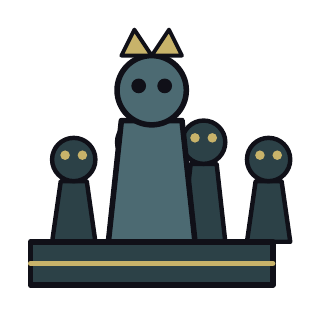
\begin{tikzpicture}[x=\Unit,y=\Unit, line join=round, line cap=round]

  % ---- the attendants, behind and smaller --------------------------------
  \foreach \i in {1,...,\Attendants} {
    \pgfmathsetmacro\x{9+(\i-1)*15}
    \pgfmathsetmacro\h{\i==2 || \i==3 ? 30 : 26}
    \fill[dark,draw=ink,line width=1.6pt] (\x,12) -- (\x+10,12) -- (\x+8,\h) -- (\x+2,\h) -- cycle;
    \fill[dark,draw=ink,line width=1.6pt] ({\x+5},{\h+5}) circle (5);
    \fill[accent] ({\x+3},{\h+6}) circle (1.1);
    \fill[accent] ({\x+7},{\h+6}) circle (1.1);
  }

  % ---- the dais -----------------------------------------------------------
  \fill[dark,draw=ink,line width=\Edge] (4,2) rectangle (60,12);
  \draw[accent,line width=1.8pt] (4,7) -- (60,7);

  % ---- the seated one, in front and in the main colour -------------------
  \fill[main,draw=ink,line width=\Edge] (22,12) -- (42,12) -- (39,40) -- (25,40) -- cycle;
  \fill[main,draw=ink,line width=\Edge] (32,47) circle (8);
  \fill[ink] (29,48) circle (1.7);
  \fill[ink] (35,48) circle (1.7);
  % A small crown, so the middle of the row is where the eye lands.
  \fill[accent,draw=ink,line width=1.4pt] (25,55) -- (28,61) -- (32,55) -- (36,61) -- (39,55) -- cycle;

\end{tikzpicture}
\end{document}
